\documentclass[a4paper,12pt]{article}

\usepackage{eurosym}
\usepackage{hyperref}
\usepackage{graphicx}
\usepackage{tikz}
\usepackage{circuitikz}
\usepackage{siunitx}
\usepackage{wrapfig}
\usepackage{listings}

\graphicspath{{./immagini/}}

\title{Arduino Gameboy}
\author{Samuele Cerea e Andrea Facoetti}

\begin{document}

\maketitle
\pagenumbering{gobble} % rimuovi i numeri dalle pagine
\lstset{language=C++}

\section{Obbiettivo}
L'obbiettivo di questo progetto \`e quello di creare una piccola console
portatile, simile al Gameboy, con un Arduino. Quindi questa console deve essere
in grado di caricare dei giochi da una cartuccia e poi eseguirli.

\section{Componenti}
\begin{center}
	\begin{tabular}{||c|c|c|c||}
		\hline
		Quantit\`a & Nome & Prezzo & Immagine \\
		\hline\hline
		1 & \href{https://www.amazon.it/dp/B01MRJR8UF}{Arduino Uno} & 15,99\euro & 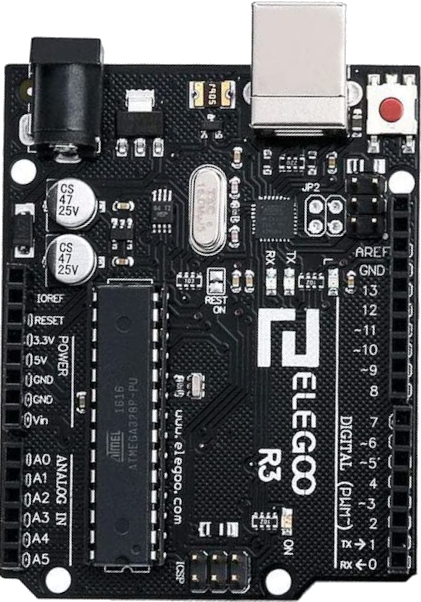
\includegraphics[width=4cm]{arduino} \\
		\hline
		1 & \href{https://www.amazon.it/dp/B07WPBQXJ9}{Kit Pulsanti} & 8,99\euro & 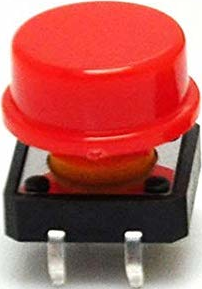
\includegraphics[width=4cm]{pulsanti} \\
		\hline
		1 & \href{https://www.amazon.it/dp/B06X1DX5WS}{Lettore Scheda SD SPI} & 5,99\euro & 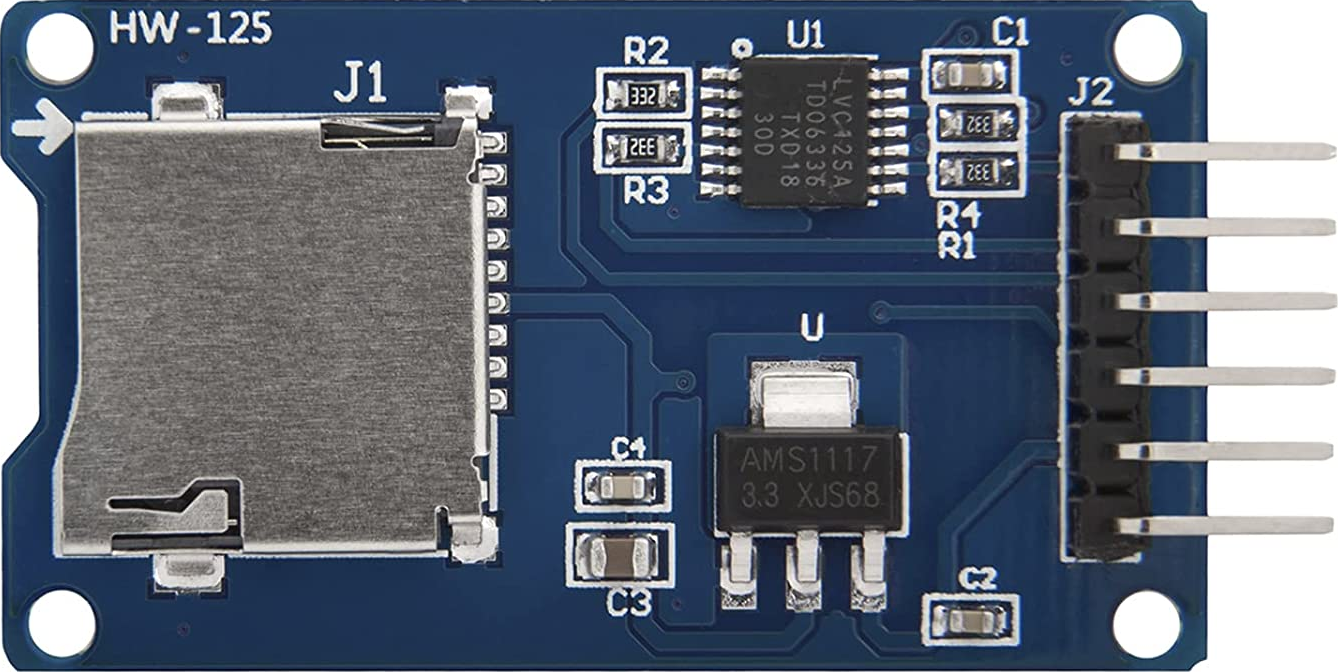
\includegraphics[width=4cm]{lettoreSD} \\
		\hline
		1 & \href{https://www.amazon.it/dp/B07G223CFP}{Display OLED 128x64 2,42 pollici SPI} & 31,99\euro & 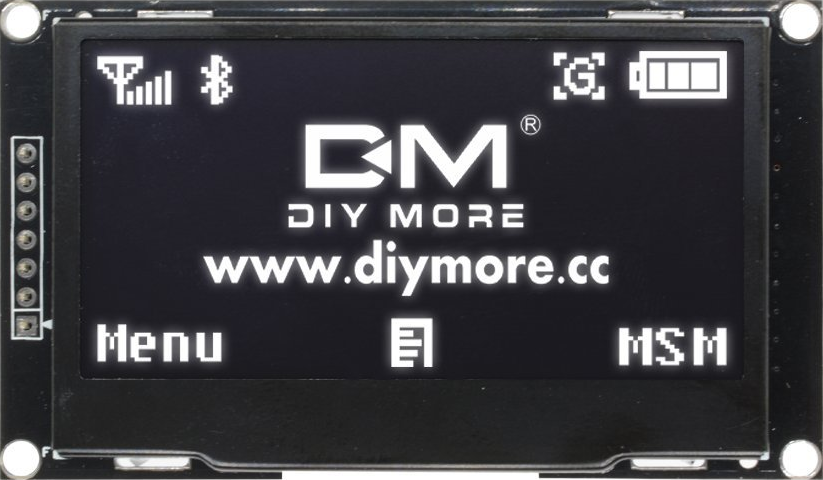
\includegraphics[width=4cm]{display} \\
		\hline
		& Cavi jumper & ~5,00\euro & \\
		\hline
		& Filo solido 22 AWG & ~10,00\euro & \\
		\hline
		3 & Breadboard & ~5,00\euro & \\
		\hline
\end{tabular}
\end{center}

\section{Circuito}
\begin{figure}[h!]
	\begin{center}
		\begin{circuitikz}
			\ctikzset{multipoles/dipchip/width=3}
			\draw (0,0) node[dipchip, num pins=26, no topmark, hide numbers, draw only pins={4-9, 14-26}](C){Arduino};
			\node [right, font=\tiny] at (C.bpin 4) {Pin A0};
			\node [right, font=\tiny] at (C.bpin 5) {Pin A1};
			\node [right, font=\tiny] at (C.bpin 6) {Pin A2};
			\node [right, font=\tiny] at (C.bpin 7) {Pin A3};
			\node [right, font=\tiny] at (C.bpin 8) {Pin A4};
			\node [right, font=\tiny] at (C.bpin 9) {Pin A5};

			\node [left, font=\tiny] at (C.bpin 26) {Pin 0};
			\node [left, font=\tiny] at (C.bpin 25) {Pin 1};
			\node [left, font=\tiny] at (C.bpin 24) {Pin 2};
			\node [left, font=\tiny] at (C.bpin 23) {Pin 3};
			\node [left, font=\tiny] at (C.bpin 22) {Pin 4};
			\node [left, font=\tiny] at (C.bpin 21) {Pin 5};
			\node [left, font=\tiny] at (C.bpin 20) {Pin 6};
			\node [left, font=\tiny] at (C.bpin 19) {Pin 7};
			\node [left, font=\tiny] at (C.bpin 18) {Pin 9};
			\node [left, font=\tiny] at (C.bpin 17) {Pin 10};
			\node [left, font=\tiny] at (C.bpin 16) {Pin 11};
			\node [left, font=\tiny] at (C.bpin 15) {Pin 12};
			\node [left, font=\tiny] at (C.bpin 14) {Pin 13};


			\draw (C.pin 4) -- ++(-2.0, 0) to [nopb] ++(-2, 0) node[ground]{};
			\draw (C.pin 5) -- ++(-.5, 0) -- ++(0, -2) -- ++(-1.5, 0) to [nopb] ++(-2, 0) node[ground]{};
			\draw (C.pin 6) -- ++(-1.0, 0) to [nopb] ++(-2, 0) node[ground]{};
			\draw (C.pin 7) -- ++(-3.5, 0) to [nopb] ++(-2, 0) node[ground]{};
		\end{circuitikz}
	\end{center}
\end{figure}

\subsection{Leggere input di un bottone}
\begin{wrapfigure}{l}{0.25\textwidth}
	\begin{circuitikz}
		\draw 
			(0, 0) [short, *-o] node[right]{\qty{5}{\volt}} 
			to [R, l_=\qty{10}{\kilo\ohm}] (0, -2.5)
			to [nopb, *-] (0, -5) 
			to node[ground]{} (0, -5)
			(0, -2.5) to [short, *-o] (1.5, -2.5) node[right]{Pin};
	\end{circuitikz}
	\caption{Pulsante in configurazione pull-up}
\end{wrapfigure}
Per leggere lo stato di un bottone \`e necessaria una configurazione pull-up o
pull-down per evitare situazioni in cui lo stato del pin di input \`e indefinito.
\\
Sulla sinistra \`e disegnato un pulsante in configurazione pull-up, e si pu\`o
osservare che quando il pulsante \`e aperto il pin sar\`a connesso ai 5 volt
attraverso la resistenza, questo assicura che il pin ha uno stato HIGH quando il
pulsante non \`e premuto. Quando si preme il pulsante il pin viene connesso
anche al ground impostando lo stato logico di LOW, inoltre la resistenza limita
la corrente che passa tra il 5 volt e il ground. Quindi la resistenza deve avere
un valore sufficentemente grande in modo da non sprecare corrente eccessiva, ma
deve comunque far passare abbastanza corrente per permettere all'Arduino di
rilevare lo stato logico HIGH quando il pulsante \`e aperto.

\section{Codice}
Il codice si trova su github \href{https://github.com/samu698/Arduino}{samu698/Arduino}
Questo progetto ha due giochi snake ed una replica del gioco del dinosauro di
chrome, il codice di questi due si trova in due file diversi snake.ino e
dino.ino.
\\
Questi file sono suddivisi in due parti una uguale ed una specifica al gioco, la
prima parte del codice svolge varie funzioni necessarie per entrambi i giochi:
\begin{itemize}
	\item Definizione di costanti come il numero dei pin e la dimensione dello schermo
	\item Inizializzazione dello schermo e dei pin
	\item Lettura dello stato dei bottoni
	\item definire la frequenza di aggiornamento dello schermo
\end{itemize}
La parte fissa del codice definisce due funzioni \verb|setup()| e \verb|loop()|
dove la prima verr\`a chiamata quando l'Arduino si attiva e la seconda verr\`a
chiamata ripetutamente dopo che viene eseguito la funzione setup.
\\
Queste due funzioni richiedo la presenza due funzioni \verb|gameSetup()| e
\verb|gameLoop()| in cui la prima svolger\`a l'Inizializzazione del gioco e la
seconda viene chiamata ogni frame per aggiornare lo stato del gioco e disegnare
sullo schermo.

\subsection{Leggere lo stato dei pulsanti}
Lo stato dei pulsanti viene letto ripetutamente mentre il codice aspetta tra un
frame ed il successivo salvando lo stato dei pulsanti in due variabili
\verb|btnsPressed| \verb|btnsHeld| dove la prima indica quali pulsanti sono
stati premuti quel frame e la seconda quali pulsanti sono tenuti premuti.
\\
Per ridurre l'use della memoria lo stato dei pulsanti \`e salvato nei bit di 
queste variabili. Grazie alle macro \verb|setBit(v, x)|, \verb|resetBit(v, x)|
e \verb|getBit(v, x)| \`e possibile scrivere, cancellare e leggere il bit in
posizione x della variabile v.
\\
Le costanti \verb|UP_BTN|, \verb|DOWN_BTN|, \verb|RIGHT_BTN| e \verb|LEFT_BTN|
indicano a quale bit corrisponde quale pulsante. Quindi per leggere set il
pulsante UP \`e stato premuto si pu\`o usare il codice:
\begin{lstlisting}
getBit(btnsPressed, UP_BTN)
\end{lstlisting}

\subsection{Il bootloader}
Il bootloader \`e del codice che si trova nella sezione finale della memoria
dell'Arduino e solitamente permette di caricare i programmi quando viene
connesso al computer. \`E possibile modificare questo codice cambiare il
funzionamento dell'Arduino.
\\
Per questo progetto i giochi devono essere caricati da una scheda SD quindi il
bootloader, al posto di caricare il codice dal computer attraverso una
comunicazione seriale, li dovr\`a caricare da una scheda SD per questo \`e
possibile utilizzare il bootloader \href {https://github.com/zevero/avr_boot}{avr-boot di zevero}
su github.
\subsubsection{Come programmere il bootloader}
Caricare il bootloader sull'Arduino richiede l'utilizzo di un'altro dispositivo,
il programmatore, in quanto il bootloader non pu\`o riscrivere se stesso.
\\
Il programmatore da noi utilizzato \`e un'altro Arduino su cui viene caricato il
codice che si pu\`o trovare nella sezione esempi dell'Arduino IDE sotto la
sezione Arduino ISP.
\\
Le due schede devono essere connesse come nel diagramma seguente, e poi sempre
dalla IDE Arduino \`e possibile caricare il bootloader.
% TODO: inserisci il diagramma
\subsection{Caricare il codice sulla scheda SD}
Il bootloader quando l'Arduino viene resettato premendo il pulsante controlla
che sulla scheda SD ci sia un file chiamato "FIRMWARE.BIN" (case-sensitive) e
carica il codice presente al suo interno.
\\
Il questo file si pu\`o ottenere utilizzando l'Arduino IDE per produrre un file
.hex dal codice del gioco e poi utilizzare il comando seguente per convertire il
file nel formato corretto
\begin{lstlisting}
avr-objcopy -I ihex -O binary <INPUT>.hex FIRMWARE.BIN
\end{lstlisting}
% TODO: immagini arduino IDE

\section{Risorse e librerie utilizzate}
% TODO

\end{document}
